\documentclass[12pt]{extarticle}
%Some packages I commonly use.
\usepackage[english]{babel}
\usepackage{framed}
\usepackage[normalem]{ulem}
\usepackage{amsmath}
\usepackage{amsthm}
\usepackage{amssymb}
\usepackage{amsfonts}
\usepackage{enumerate}
\usepackage[top=1 in,bottom=1in, left=1 in, right=1 in]{geometry}
\usepackage{graphicx}
\usepackage[utf8]{inputenc} % Required for inputting international characters
\usepackage[T1]{fontenc} % Output font encoding for international characters
\usepackage{mathpazo} % Palatino font
\usepackage{xfrac}% http://ctan.org/pkg/xfrac

%A bunch of definitions that make my life easier
\newcommand{\matlab}{{\sc Matlab} }
\newcommand{\cvec}[1]{{\mathbf #1}}
\newcommand{\rvec}[1]{\vec{\mathbf #1}}
\newcommand{\ihat}{\hat{\textbf{\i}}}
\newcommand{\jhat}{\hat{\textbf{\j}}}
\newcommand{\khat}{\hat{\textbf{k}}}
\newcommand{\minor}{{\rm minor}}
\newcommand{\trace}{{\rm trace}}
\newcommand{\spn}{{\rm Span}}
\newcommand{\rem}{{\rm rem}}
\newcommand{\ran}{{\rm range}}
\newcommand{\range}{{\rm range}}
\newcommand{\mdiv}{{\rm div}}
\newcommand{\proj}{{\rm proj}}
\newcommand{\R}{\mathbb{R}}
\newcommand{\N}{\mathbb{N}}
\newcommand{\Q}{\mathbb{Q}}
\newcommand{\Z}{\mathbb{Z}}
\newcommand{\<}{\langle}
\newcommand\tab[1][1cm]{\hspace*{#1}}
\newcommand{\attn}[1]{\textbf{#1}}
\newcommand{\bproof}{\bigskip {\bf Proof. }}
\newcommand{\eproof}{\hfill\qedsymbol}
\newcommand{\Disp}{\displaystyle}
\newcommand{\qe}{\hfill\(\bigtriangledown\)}
\renewcommand{\>}{\rangle}
\renewcommand{\emptyset}{\varnothing}
\renewcommand*\contentsname{Summary}
\theoremstyle{definition}
\newtheorem{theorem}{Theorem}
\newtheorem{corollary}{Corollary}
\newtheorem*{definition}{Definition}
\newtheorem*{example}{Example}
\newtheorem*{note}{Note}
\newtheorem{exercise}{Exercise}
\setlength{\columnseprule}{1 pt}

\title{Light Sensing Circuit}
\author{Group 1}
\date{May $8^{th}$, 2019}

\begin{document}

%----------------------------------------------------------------------------------------
%	TITLE PAGE
%----------------------------------------------------------------------------------------

\begin{titlepage} % Suppresses displaying the page number on the title page and the subsequent page counts as page 1
	\newcommand{\HRule}{\rule{\linewidth}{0.5mm}} % Defines a new command for horizontal lines, change thickness here
	
	\center % Centre everything on the page
	
	%------------------------------------------------
	%	Headings
	%------------------------------------------------
	
	\textsc{\LARGE HO CHI MINH CITY UNIVERSITY OF TECHNOLOGY}\\[0.25cm] % Main heading such as the name of your university/college

	\begin{figure}[ht]
		\begin{center}
			
			
\includegraphics[scale=0.12]{logobk.png}\\
	
		\end{center}
		
		
	\end{figure}
	%------------------------------------------------
	%	Title
	%------------------------------------------------
	
	\HRule\\[0.4cm]
	
	{\huge\bfseries Report Project 1: A LIGHT SENSING CIRCUIT}\\[0.4cm] % Title of your document
	
	\HRule\\[0.5cm]
	\begin{figure}[ht]
		\begin{center}
			
			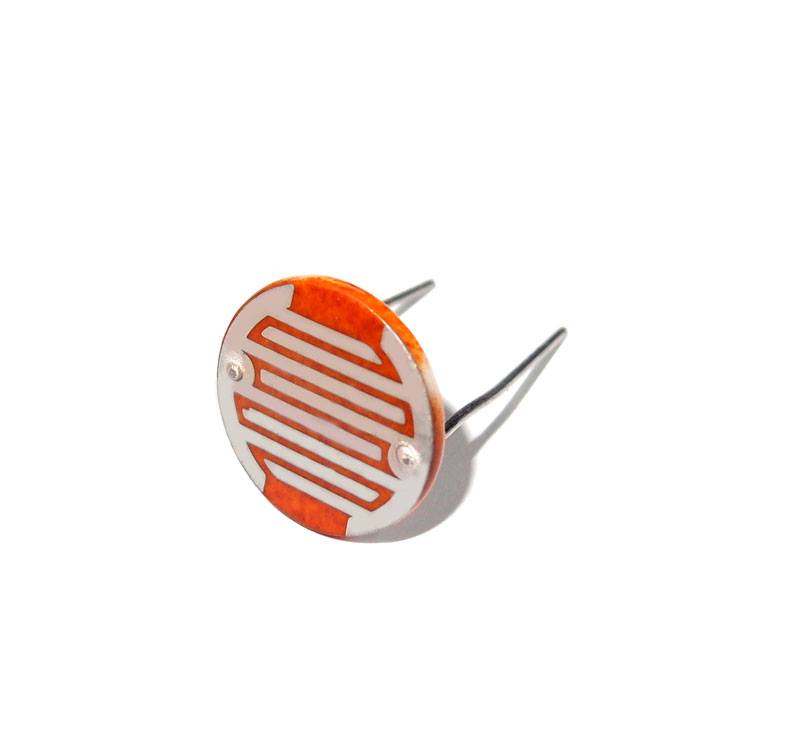
\includegraphics[scale=0.2]{sensor.jpg}\\
			
		\end{center}
	\end{figure}
	%------------------------------------------------
	%	Author(s)
	%------------------------------------------------
	
	\begin{minipage}{0.5\textwidth}
		\begin{flushleft}
			\large
			\textit{Lecturer: }\\
			 \textsc{Nguyen Tran Huu Nguyen} % Your name
		\end{flushleft}
	\end{minipage}
	~
	\begin{minipage}{0.4\textwidth}
		\begin{flushright}
			\large
			\textit{Course:}\\
			 \textsc{Electronic Devices and Circuit(Lab)} % Supervisor's name
		\end{flushright}
	\end{minipage}
	
	% If you don't want a supervisor, uncomment the two lines below and comment the code above
	%{\large\textit{Author}}\\
	%John \textsc{Smith} % Your name
	
	%------------------------------------------------
	%	Date
	%------------------------------------------------
	
	\vfill\vfill\vfill % Position the date 3/4 down the remaining page
	
	{\large May $8^{th}$, 2019} % Date, change the \today to a set date if you want to be precise
	
	%------------------------------------------------
	%	Logo
	%------------------------------------------------
	
	%\vfill\vfill
	%\includegraphics[width=0.2\textwidth]{placeholder.jpg}\\[1cm] % Include a department/university logo - this will require the graphicx package
	 
	%----------------------------------------------------------------------------------------
	
	\vfill % Push the date up 1/4 of the remaining page
	
\end{titlepage}

%----------------------------------------------------------------------------------------

\begin{center}
{\huge\bfseries GROUP MEMBERS}\\[1cm]

\end{center}
	\begin{minipage}{0.5\textwidth}
		\begin{flushleft}
			\large
			\textit{{\huge\bfseries NAME}\\[0.5cm]}
			 \textsc{{Ngo Qui Thu}\\[0.2cm]}
			 \textsc{{Nguyen Huu Gia Huy}\\[0.2cm]}
			 \textsc{{Tran Hoang Viet Long}\\[0.2cm]}
			 \textsc{{Truong Van Quang Dat}\\[0.2cm]}
			 \textsc{{Pham Le The Anh}\\[0.2cm]}
			 \textsc{{Vuong Le Huy}\\[0.2cm]}
		\end{flushleft}
	\end{minipage}
	~
	\begin{minipage}{0.5\textwidth}
		\begin{flushright}
			\large
			\textit{{\huge\bfseries ID}\\[0.5cm]}
			 \textsc{{1652595}\\[0.2cm]}
			 \textsc{{1652242}\\[0.2cm]}
			 \textsc{{1652350}\\[0.2cm]}
			 \textsc{{1652142}\\[0.2cm]}
			 \textsc{{1652026}\\[0.2cm]}
			 \textsc{{1652252}\\[0.2cm]}
		\end{flushright}
	\end{minipage}
\clearpage
%----------------------------------------------------------------------------------------

%{\huge\bfseries LIST OF CONTENTS:}\\[1cm]		

{\large\tableofcontents}


\maketitle

\section{$R_1$, $R_2$, $R_3$ Calculation and Power Evaluation}
\subsection{$R_1$, $R_2$ and $R_3$ Calculation}
\begin{normalsize}
According to Kirchoff's Voltage Laws (KVL), we have the following equation:
\begin{align*}
&-12 + V_{R_3} + 3V_F = 0\\
&\Longrightarrow V_{R_3} = 12 - 3V_F\\
&\Longrightarrow R_3 = \frac{V_{R_3}}{I_{sccR_3}} = \frac{V_{R_3}}{I_F} = \frac{12 - 3V_F}{I_F}(\Omega)
\end{align*}
$\bullet$ In case of $V_F  = 3V \longrightarrow 3.4V$.
\begin{align*}
&I_F = 25mA - 30mA\\
&\Longrightarrow R_3 \in \left[\frac{12 - 3x3.4}{30x10^{-3}} ; \frac{12 - 3x3}{25x10^{-3}}\right]\\
&\iff R_3 \in [60 ; 120] (\Omega)
\end{align*}
$\bullet$ Choose $R_L = 40000\Omega$, we have the following expression:
\begin{align*}
&I_{R_2} = I_L = \frac{0.7}{40000} = 1.78x10^6(A)
\end{align*}
Results below can be extracted by appling kirchoff's Voltage Laws. 
\begin{align*}
&-12 + V_{R_2} + V_{R_L} = 0\\
&\Longrightarrow V_{R_2} = 12 - V_{R_L} = 12 - 0.7 = 11.3(V)\\
&\Longrightarrow R_2 = \frac{V_{R_2}}{I_{R_2}} = 645414 (\Omega)
\end{align*}
Base on the value of $R_L$ measured by VOM, the following results can be infered:
\begin{align*}
&R_2 = \frac{11.3}{\frac{0.7}{R_L}} = \frac{11.3 X R_L}{0.7} = 12.14R_L (\Omega)
\end{align*}
Applying Kirchoff's Laws:
\begin{align*}
&I_{R_1} = I_{R_2} + I_{R_3}\\
&\Longrightarrow I_{R_1} = I_{R_2} + I_F\\
&\Longrightarrow I_{R_1} = \frac{0.7}{R_2} + I_F\\
&\Longrightarrow I_{R_1} \in [0.025 ; 0.03] (A)
\end{align*}
Measurement results in laboratory reportedly show that voltage at the two ends of the capacitor peaks at $12\sqrt{2} (V)$.
\begin{align*}
V_{0C} = 12\sqrt{2} (V)
\end{align*}
$\bullet$ In case of the worst situation when $V_{DC} = 18.8(V)$ so that $R_1$ is going to be designed in a way such that $V_{DC} = 12 (V)$.
\begin{align*}
&\Longrightarrow R_1 = \frac{18.8 - 12}{I_{R_1}}\\
&\Longrightarrow R_1 \in [227 ; 275](\Omega)
\end{align*}
\subsection{Power Evaluation}
Given the fact that, the circuit is designed to operate normally at the 12V voltage level. While the value of $V_{AC}$ reportedly stations at 14V ($V_{AC} = 14V$), which resulted in the following value:
\begin{align*}
&V_{DC without R_1} =  18.8(V)
\end{align*}
That result leads to the below calculations:
\begin{align*}
&\bullet V_{R_1} = 18.8 - 12 = 6.8(V)\\
&\bullet P_{R_1} = \frac{(18\sqrt{2} - R_1)^2}{R_1}\\
&\Longrightarrow P_{R_1} \in [0.168 ; 0.204](W)
\end{align*}
Given the Safe Factor to be $\geq 1.5$. If $V_{AC}$ exceeds the common voltage of $12V$, the circuit can withstand up to $18.8V$ before suffering structural damages.
\begin{align*}
&P_{R_1} = \frac{(18\sqrt{2} - 12)^2}{R_1}\\
&\Longrightarrow P_{R_1} \in [0.7 ; 0.8](W)
\end{align*}
$\bullet$ Choose $R_1 = 250\Omega, 0.5W$ in order to guarantee that the circuit can withstand the voltage up to 1.5 times higher than the normal designed voltage.
\section{Proceeding Steps}
\subsection{Components List} 
\tab - 100$\Omega$, $\sfrac{1}{4}W$ Resistor\\
\tab - 150$\Omega$, $0.5W$ Resistor\\
\tab - 470$K\Omega$, $\sfrac{1}{4}W$ Resistor\\
\tab - Light Sensoring Resistor\\
\tab - Zener Diode\\
\tab - C1815 NPN Transistor\\
\tab - 3 LEDs\\
\tab - 4 Diodes
\subsection{$R_1$, $R_2$, $R_3$ Build Method} 
%Ve 2 mach R1 R2 dum t nha m
\subsubsection{$R_1$ Component}
Only 150$\Omega$, $0.5W$ Resistor is avalable. Thus system of $R_1$ resistors are built as follow in order to get the exactly calculated value $R_1 = 250(\Omega)$.
\subsubsection{$R_2$ Component}
System of $R_2$ resistors are built as follow in order to get the exactly calculated value $R_2 = 645(K\Omega)$ .
\subsubsection{$R_3$ Component}
\tab $R_3 = R = 100(\Omega)$.
\end{normalsize}
\end{document}